\chapter{Package \texttt{noisemodels}}

This is a module that generates noisemodels of various interferometers
and helps run simple filtering of data simulated with these noise models.
The test codes can easily be generalized to filter data from real
detectors.

There are basically three test codes:
\begin{enumerate}
\item \texttt{NoisePSDTest}
\item \texttt{RandomSignal}
\item \texttt{FilterTest}
\end{enumerate}

\paragraph* {\texttt{NoisePSDTest}:} This test code makes four
successive calls to the function \texttt{LALNoiseSpectralDensity}
successively passing a pointer to the functions \texttt{LALGEOPsd,}
\texttt{LALLIGOIPsd}, \texttt{LALTAMAPsd} and \texttt {LALVIRGOPsd}.
The function \texttt{LALNoiseSpectralDensity} returns the power
spectrum in units Hz$^{-1}$ while the test code \texttt{NoisePSDTest}
outputs the amplitude spectrum in units Hz$^{-1/2}.$ The figure
below shows the output of the test  code.
\begin{center}
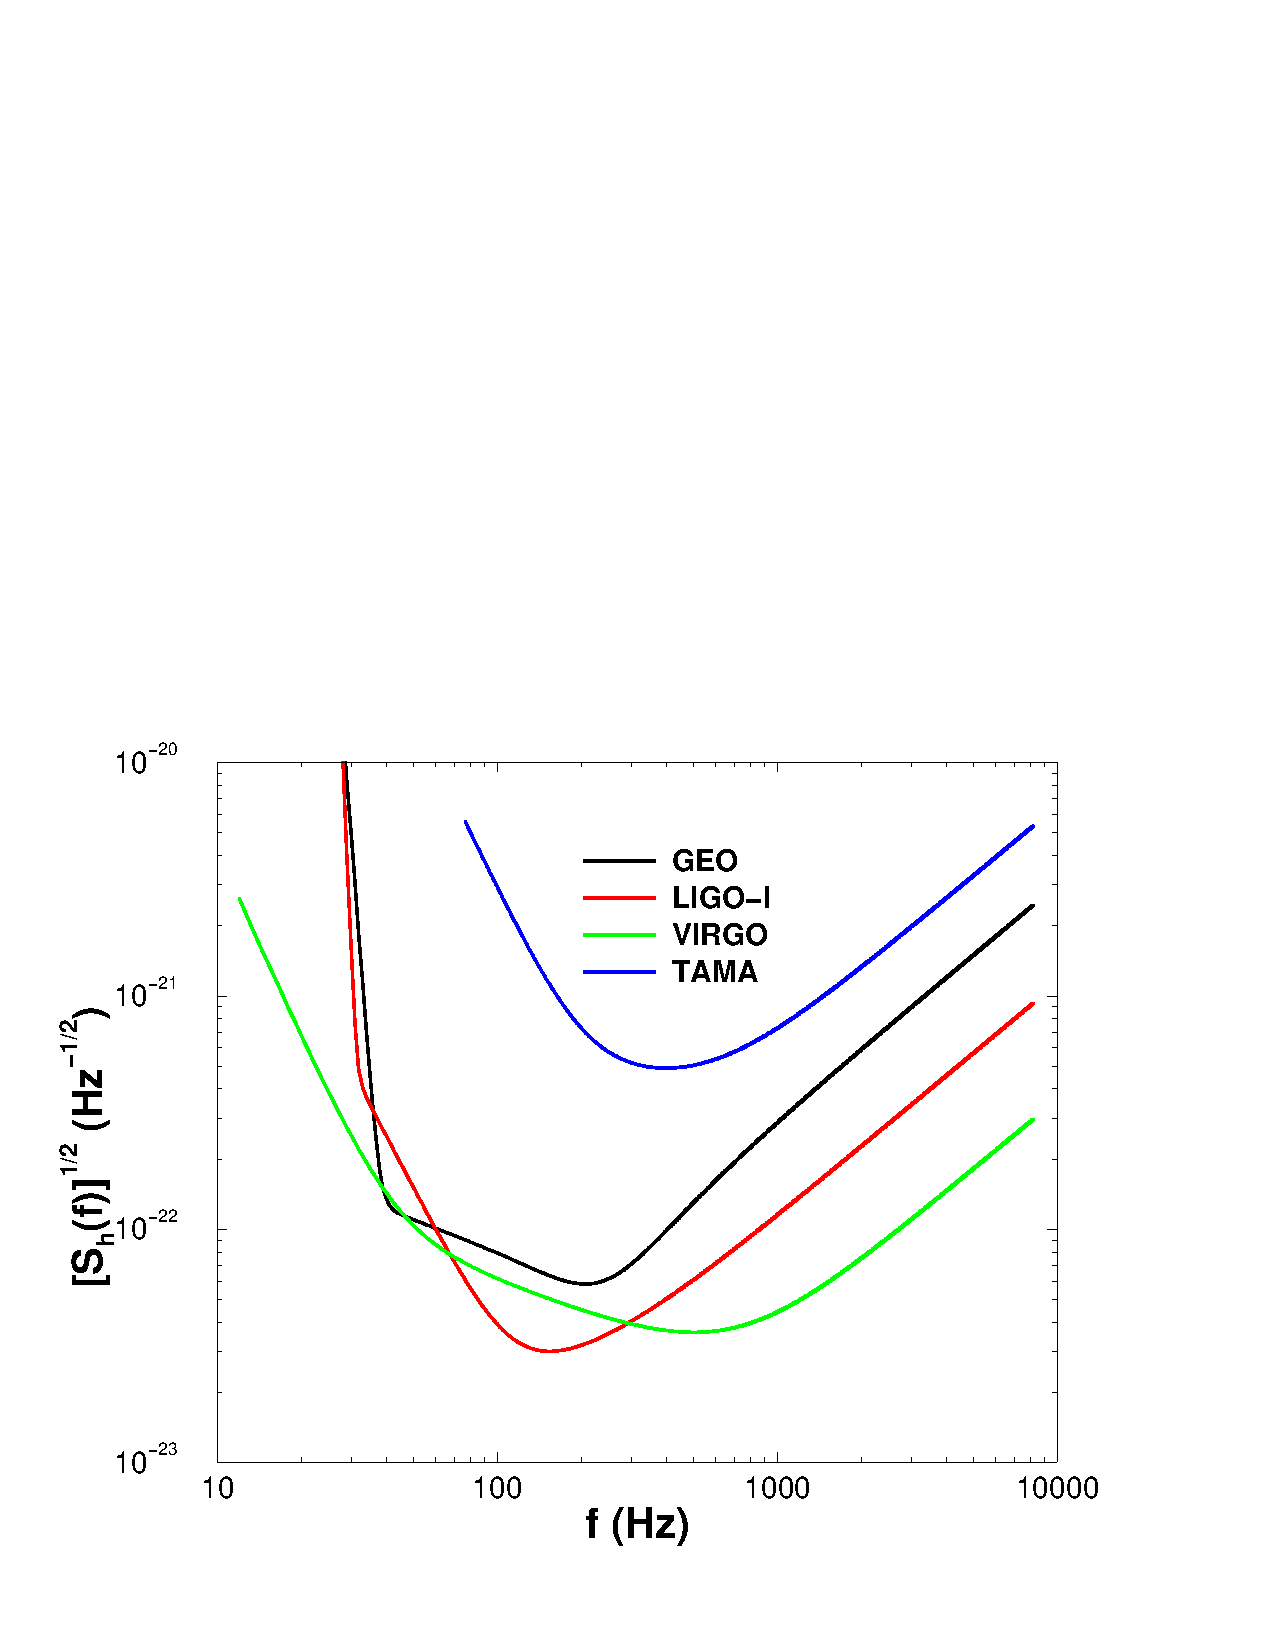
\includegraphics[angle=-90,width=4truein]{NoisePSDTest.pdf}
\end{center}

\paragraph* {\texttt{RandomSignal}:} This test code makes three
successive calls to \texttt{LALRandomInspiralSignal} generating
(1) only signal, (2) only noise and (3) signal + noise, each
time filtering the generated data with a orthogonal set of templates
whose parameters are the same as the generated signal in
cases (1) and (3) but arbitrary in the case of (2). The resulting
correlations are shown in the diagram below:
\begin{center}
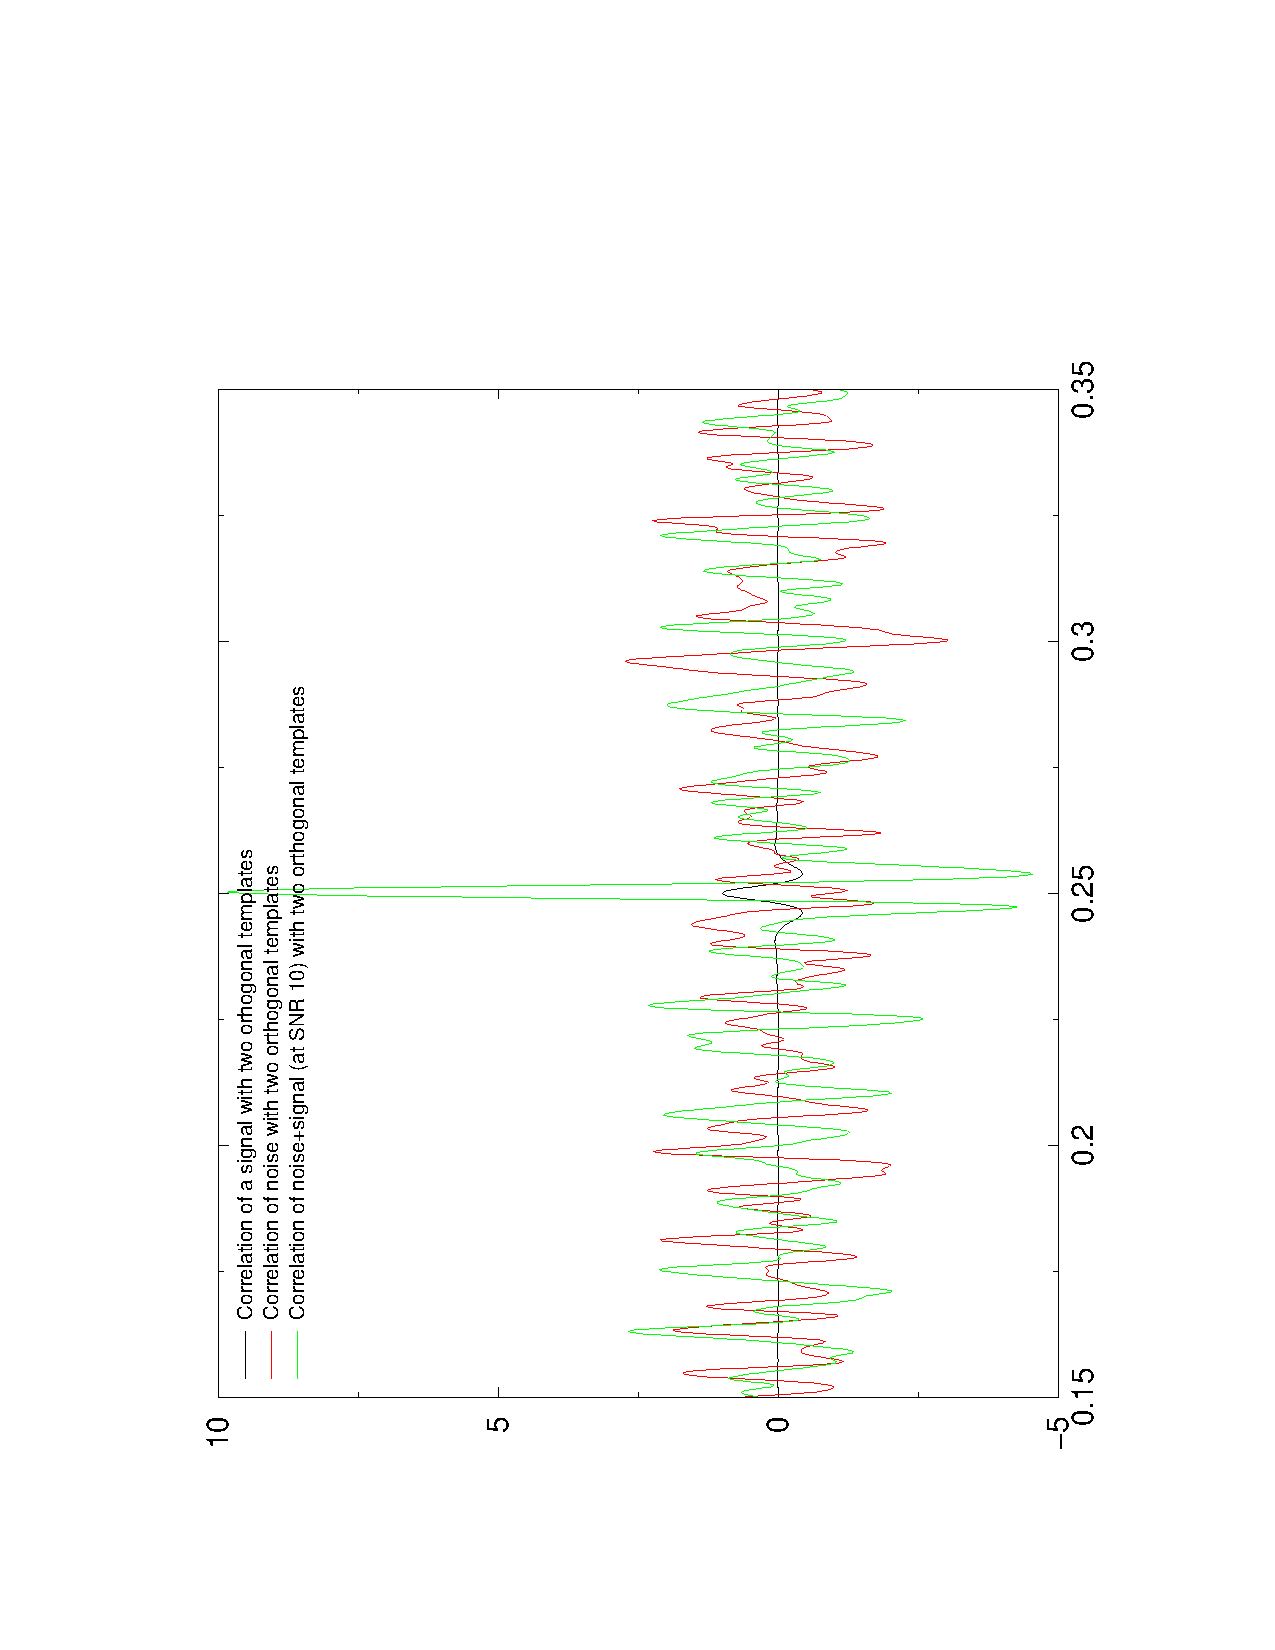
\includegraphics[angle=-90,width=4truein]{RandomSignal.pdf}
\end{center}
\paragraph* {\texttt{FilterTest}:} This test code generates
a lattice of template coordinates at a given {\it minimal match}
and for a given total maximum mass $M_{\rm max}$ and minimum of components
masses $m_{\rm min},$ it then filters signals with random parameters
with those templates that are 'close' to the signal and records
the lagest overlap obtained. The generated random signal could
be (1) only signal, (2) only noise or (3) noise + signal at a specified
SNR. For each of the signal generated the code ouputs the maximum
SNR obtained together with the parameters of the signal that was
generated. A typical run may output the following on screen in
addition to recording the output in a file named \texttt{FilterTest.outt}.

\begin{verbatim}
This test code does three things:
(a) Creates a filter bank at a certain minimal match
(b) Generates signals with random parmeters
(c) Filters each of these signals with the a subset of
    templates close to the random signal and reports the best SNR achived
Results of the run are written in FilterTest.out
#Number of Coarse Bank Templates=174
----------------------------------------------
   t0             t2        Overlap/SNR
----------------------------------------------
2.453413e+00 3.519999e-01 9.004098e+00
9.417101e-01 2.336294e-01 6.490586e+00
1.059791e+00 2.202322e-01 8.958589e+00
1.513863e+00 2.598545e-01 7.762945e+00
9.451709e-01 2.087785e-01 6.673258e+00
7.876498e-01 1.785656e-01 8.225487e+00
2.081274e+00 3.178223e-01 7.423584e+00
1.078093e+00 2.220369e-01 7.389996e+00
5.887522e-01 1.601810e-01 9.039020e+00
2.434745e+00 3.493113e-01 9.553841e+00
\end{verbatim}

\newpage\input{LALNoiseModelsH}
